\section{Background Theories} \label{sub:theories}
This project approaches AUI, extensively using the user modelling technique. ``The \emph{user model} is a representation of information about an individual user that is essential for an adaptive system to provide \emph{the adaptation effect}''\cite{brusilovsky2007user}. The theories and concepts used in this project is drawn from Brusilovsky \cite{brusilovsky2007user} and Strachan \cite{strachan2000minimalist}

This model makes it possible for the system to behave differently for different users. An adaptive system creates and maintains such data by either implicitly observing the user interaction or explicitly request the necessary data from the user or in most cases do both. The volume and or nature of the information represented in the user model of an Adaptive System, to a large extent depends on the sort of adaptation effect that the system is designed to achieve. \cite{brusilovsky2007user}.
\subsection{User Modeling}
Following on from Brusilovsky, we will look at modelling the user by distinguishing models that represent features of the user as an individual from models that represent the context of the user's work. As stated in \cite{brusilovsky2007user} the former is important to all adaptive web systems while the latter mostly concerns mobile and ubiquitous adaptive systems.From an individual user's perspective we will explore the following features:
\begin{itemize}
\item Knowledge
\item Interests
\item Goals and Tasks
\item Background
\item Individual Traits
\end{itemize}

Modeling with such features is known as feature-based user modeling as opposed to stereotype modeling. Stereotype modeling instead of using individual features, tries to categorise all users of an adaptive system into several groups known as stereotypes. This is one of the oldest approaches to user modeling. This project will use elements of this type of modeling but not extensively as feature based modeling.

\subsubsection{Knowledge}
The user's knowledge of the domain of discourse, is important. The user's knowledge is known to be a changeable feature. That is, it can increase or decrease from session to session; meaning the system has to recognise such changes and update accordingly.
\subsubsection{Interests}
This focuses on the interests of the user as individual, it is not what they know but what interests them in the domain of discourse or in a general scope and in the context of the project, items or content they would not mind to have on their screen or dashboard
\subsubsection{Goals and Task}
What is the user's goal or aim in using the system?Clearly identifying this would make it possible to formulate task models to map each goal or task and influence how the system adapts
\subsubsection{Background}
What are the user's experience outside the current domain (this project's web application)? Do they have any experience using systems that try to accomplish the same task? In the context of this project a background feature could be the user's teaching experience.
\subsubsection{Individual Traits}
This is what defines the user as an individual. While different kinds of user traits are being discussed exhaustively in psychological literature, current work on mdeling and using individual traits for personalisation focuses mostly on two groups of traits - \emph{Cognitive and learning styles} \cite{brusilovsky2007user}
\section{Methodology}
In this project we try to implement an Adaptive User Interface for a classroom managment web application for teachers. The emphasis here is on the teacher and not the student or pupils. The application is meant to aide teachers in their daily tasks and make their interactions with the system seamless.
As mention in \ref{sub:theories} this project follows the user modeling theory as reviewed and discussed by Brusilovsky \cite{brusilovsky2007user} and Strachan \cite{strachan2000minimalist}.

We have designed an online survey\cite{website:UserSurvey} to gather explicit information on some teachers; the survey has been designed to capture information such as age, sex, teaching subject,level of competency with computers, daily tasks and teaching experience. That will go into modeling or creating a general knowledge to help design a model of the system itself and to establish some use cases while designing and implementing the system.
\begin{figure}[!ht]
    \caption{Survey Questions}
    \label{fig:survey}
    \centering
    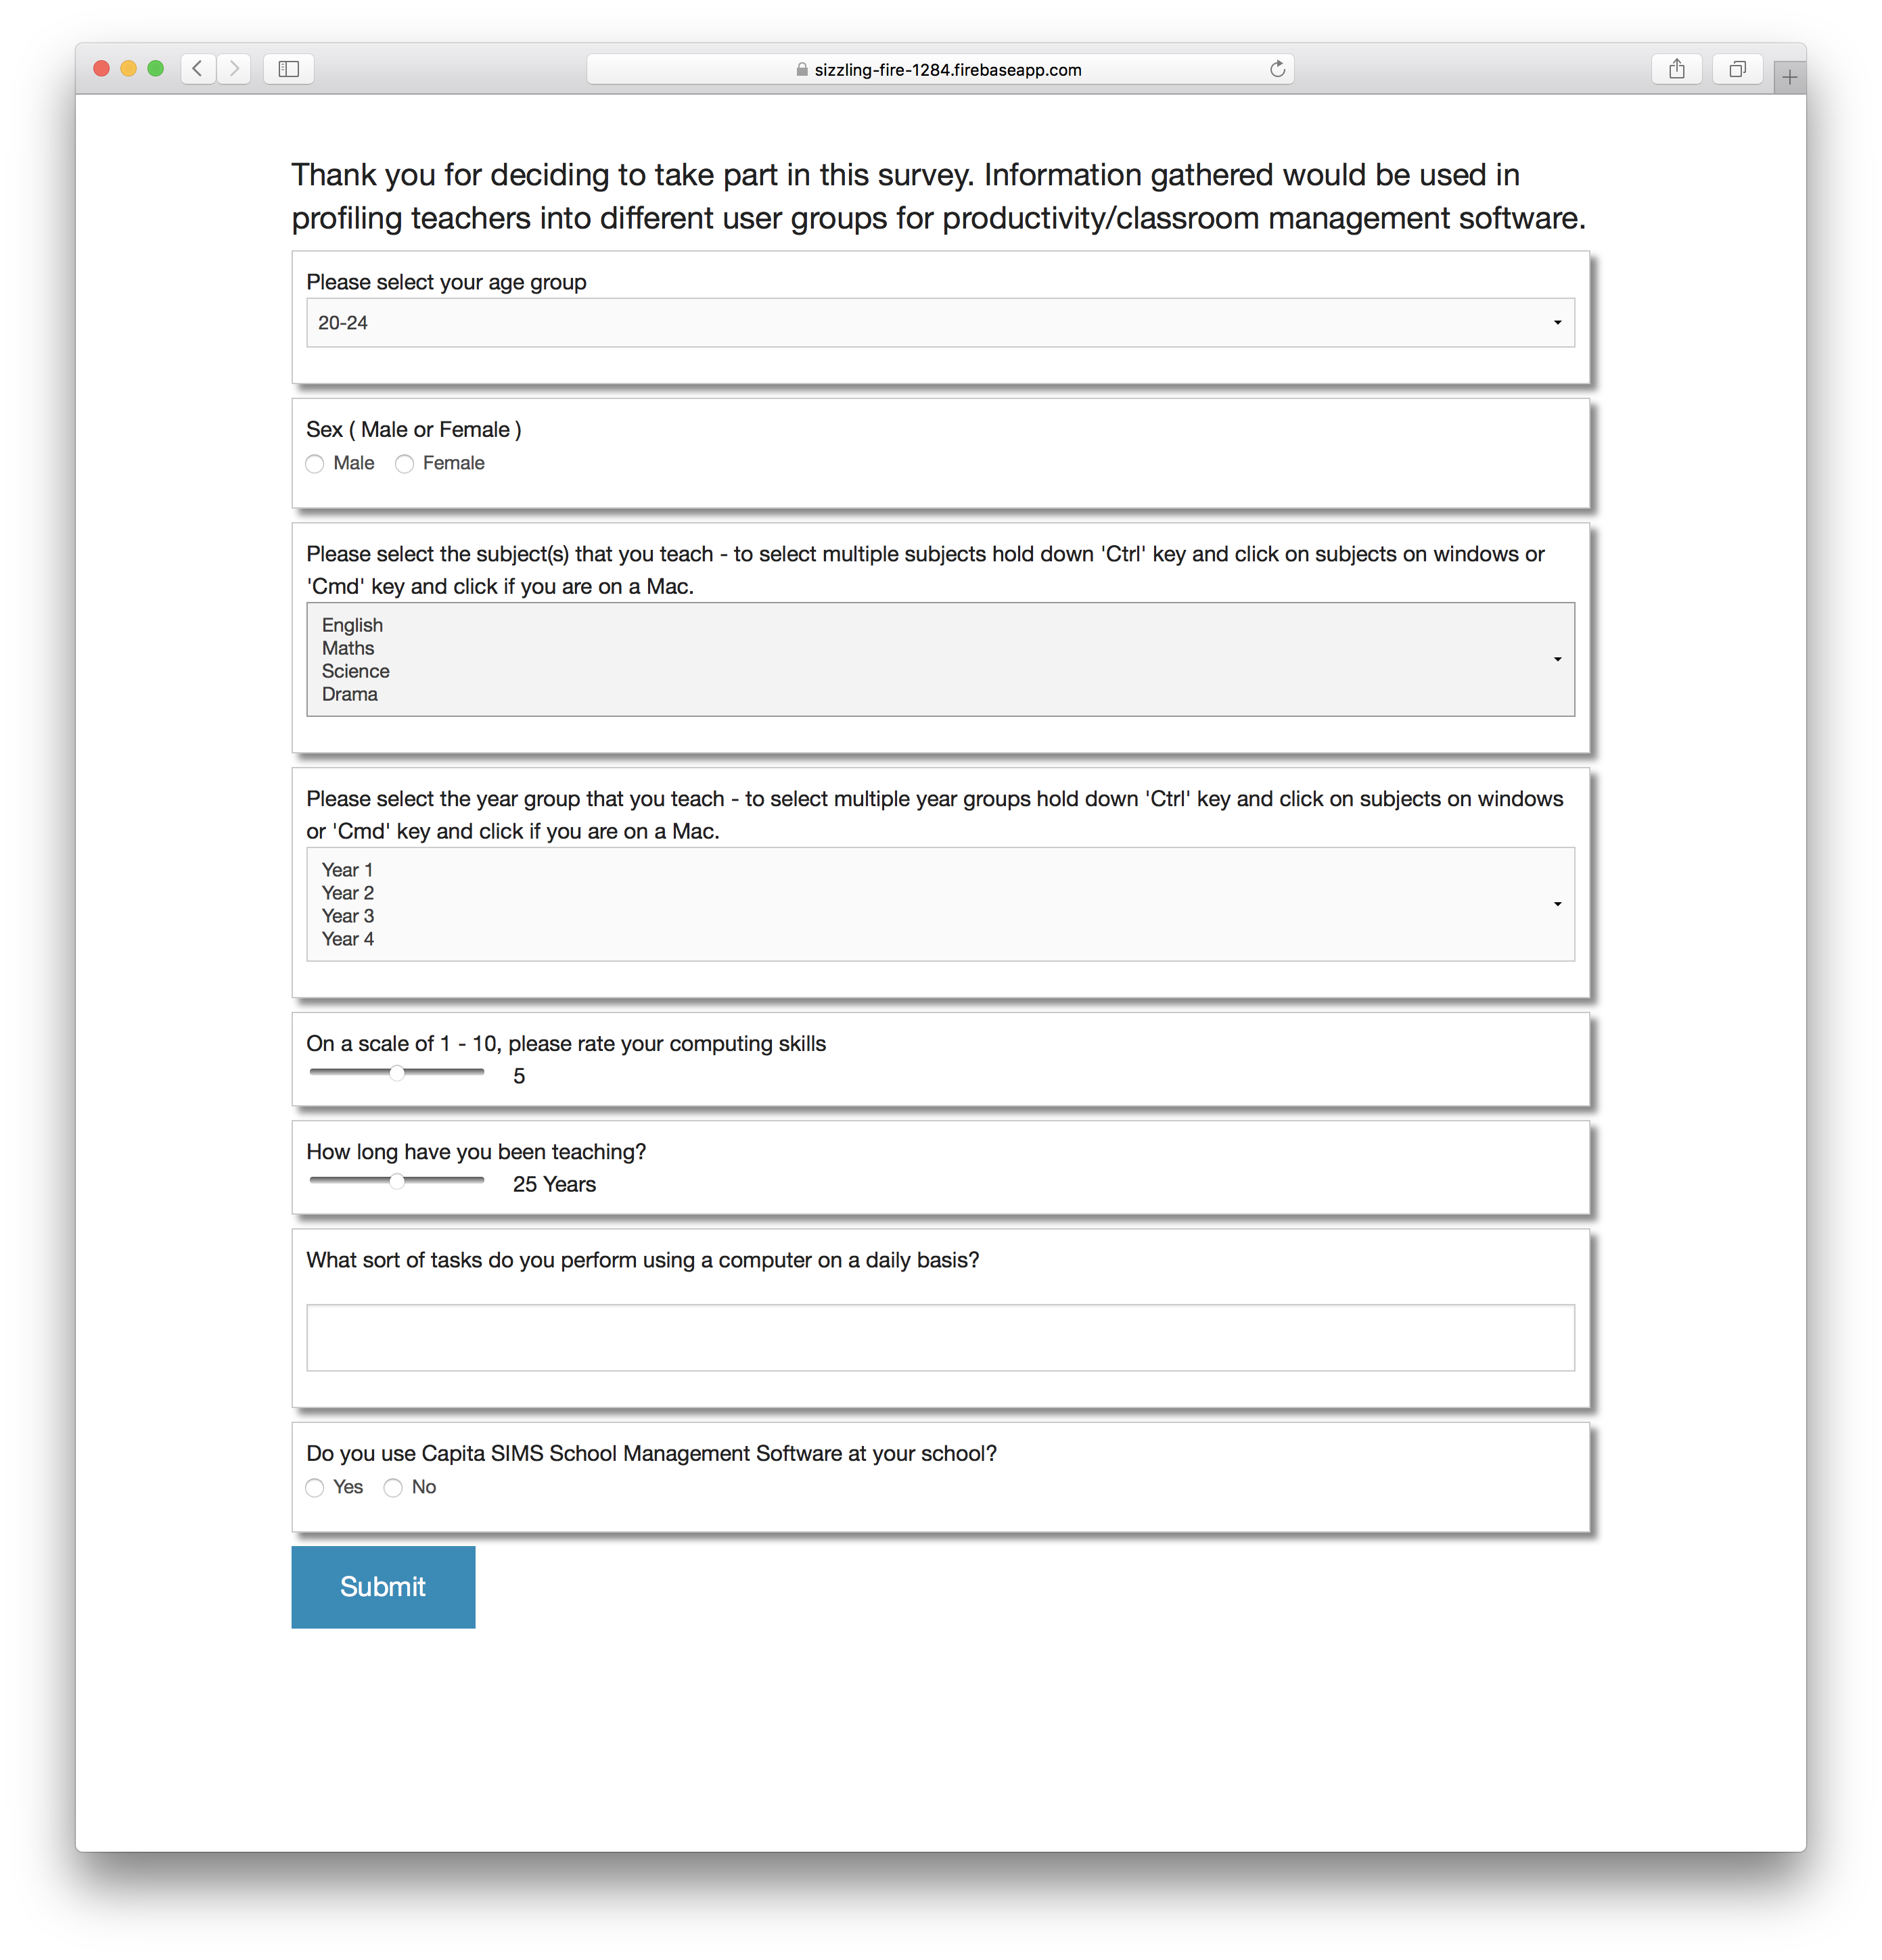
\includegraphics[scale=0.1]{figures/survey_shot}
\end{figure}

The aim of this was not to necessarily gather information for user modeling but for task modeling and from that infer what sort of tasks are prominent and among which of the sexes? Out of the 31 people that have taken part of the survey so far, 29 are women and only 2 are men. The women a percentage of the women explicitly added \emph{email and social media} to their daily tasks whereas the men, although only 2 of them made no mention of emails or social media. This will be general knowledge for the system that all female users between \textbf{25-50} should be given the feature to email or a social media platform initially whereas it should be present for the male users unless otherwise stated. \emph{stereotyping}.

Information on the various levels in computing skills recorded helps us establish a starting point of state to initialise the system in and accordingly adapt specific elements to suit the user's needs, in this case we are making use of stereotype modeling. This ensures that the system does not start off blank and then rapidly try to adapt to the user. Having gathered this information beforehand we can then start with something the user relates to and then gradually generate feature models on them.

The conclusion that can be made based on this survey with regards to teacher tasks; \emph{Planning} is a recurring task for all of them, how they go about this is something that would need to be recorded by the system by monitoring the users planning process. 
\begin{figure}[!ht]
    \caption{A number of women explicitly state emails and social media}
    \label{fig:Social}
    \centering
    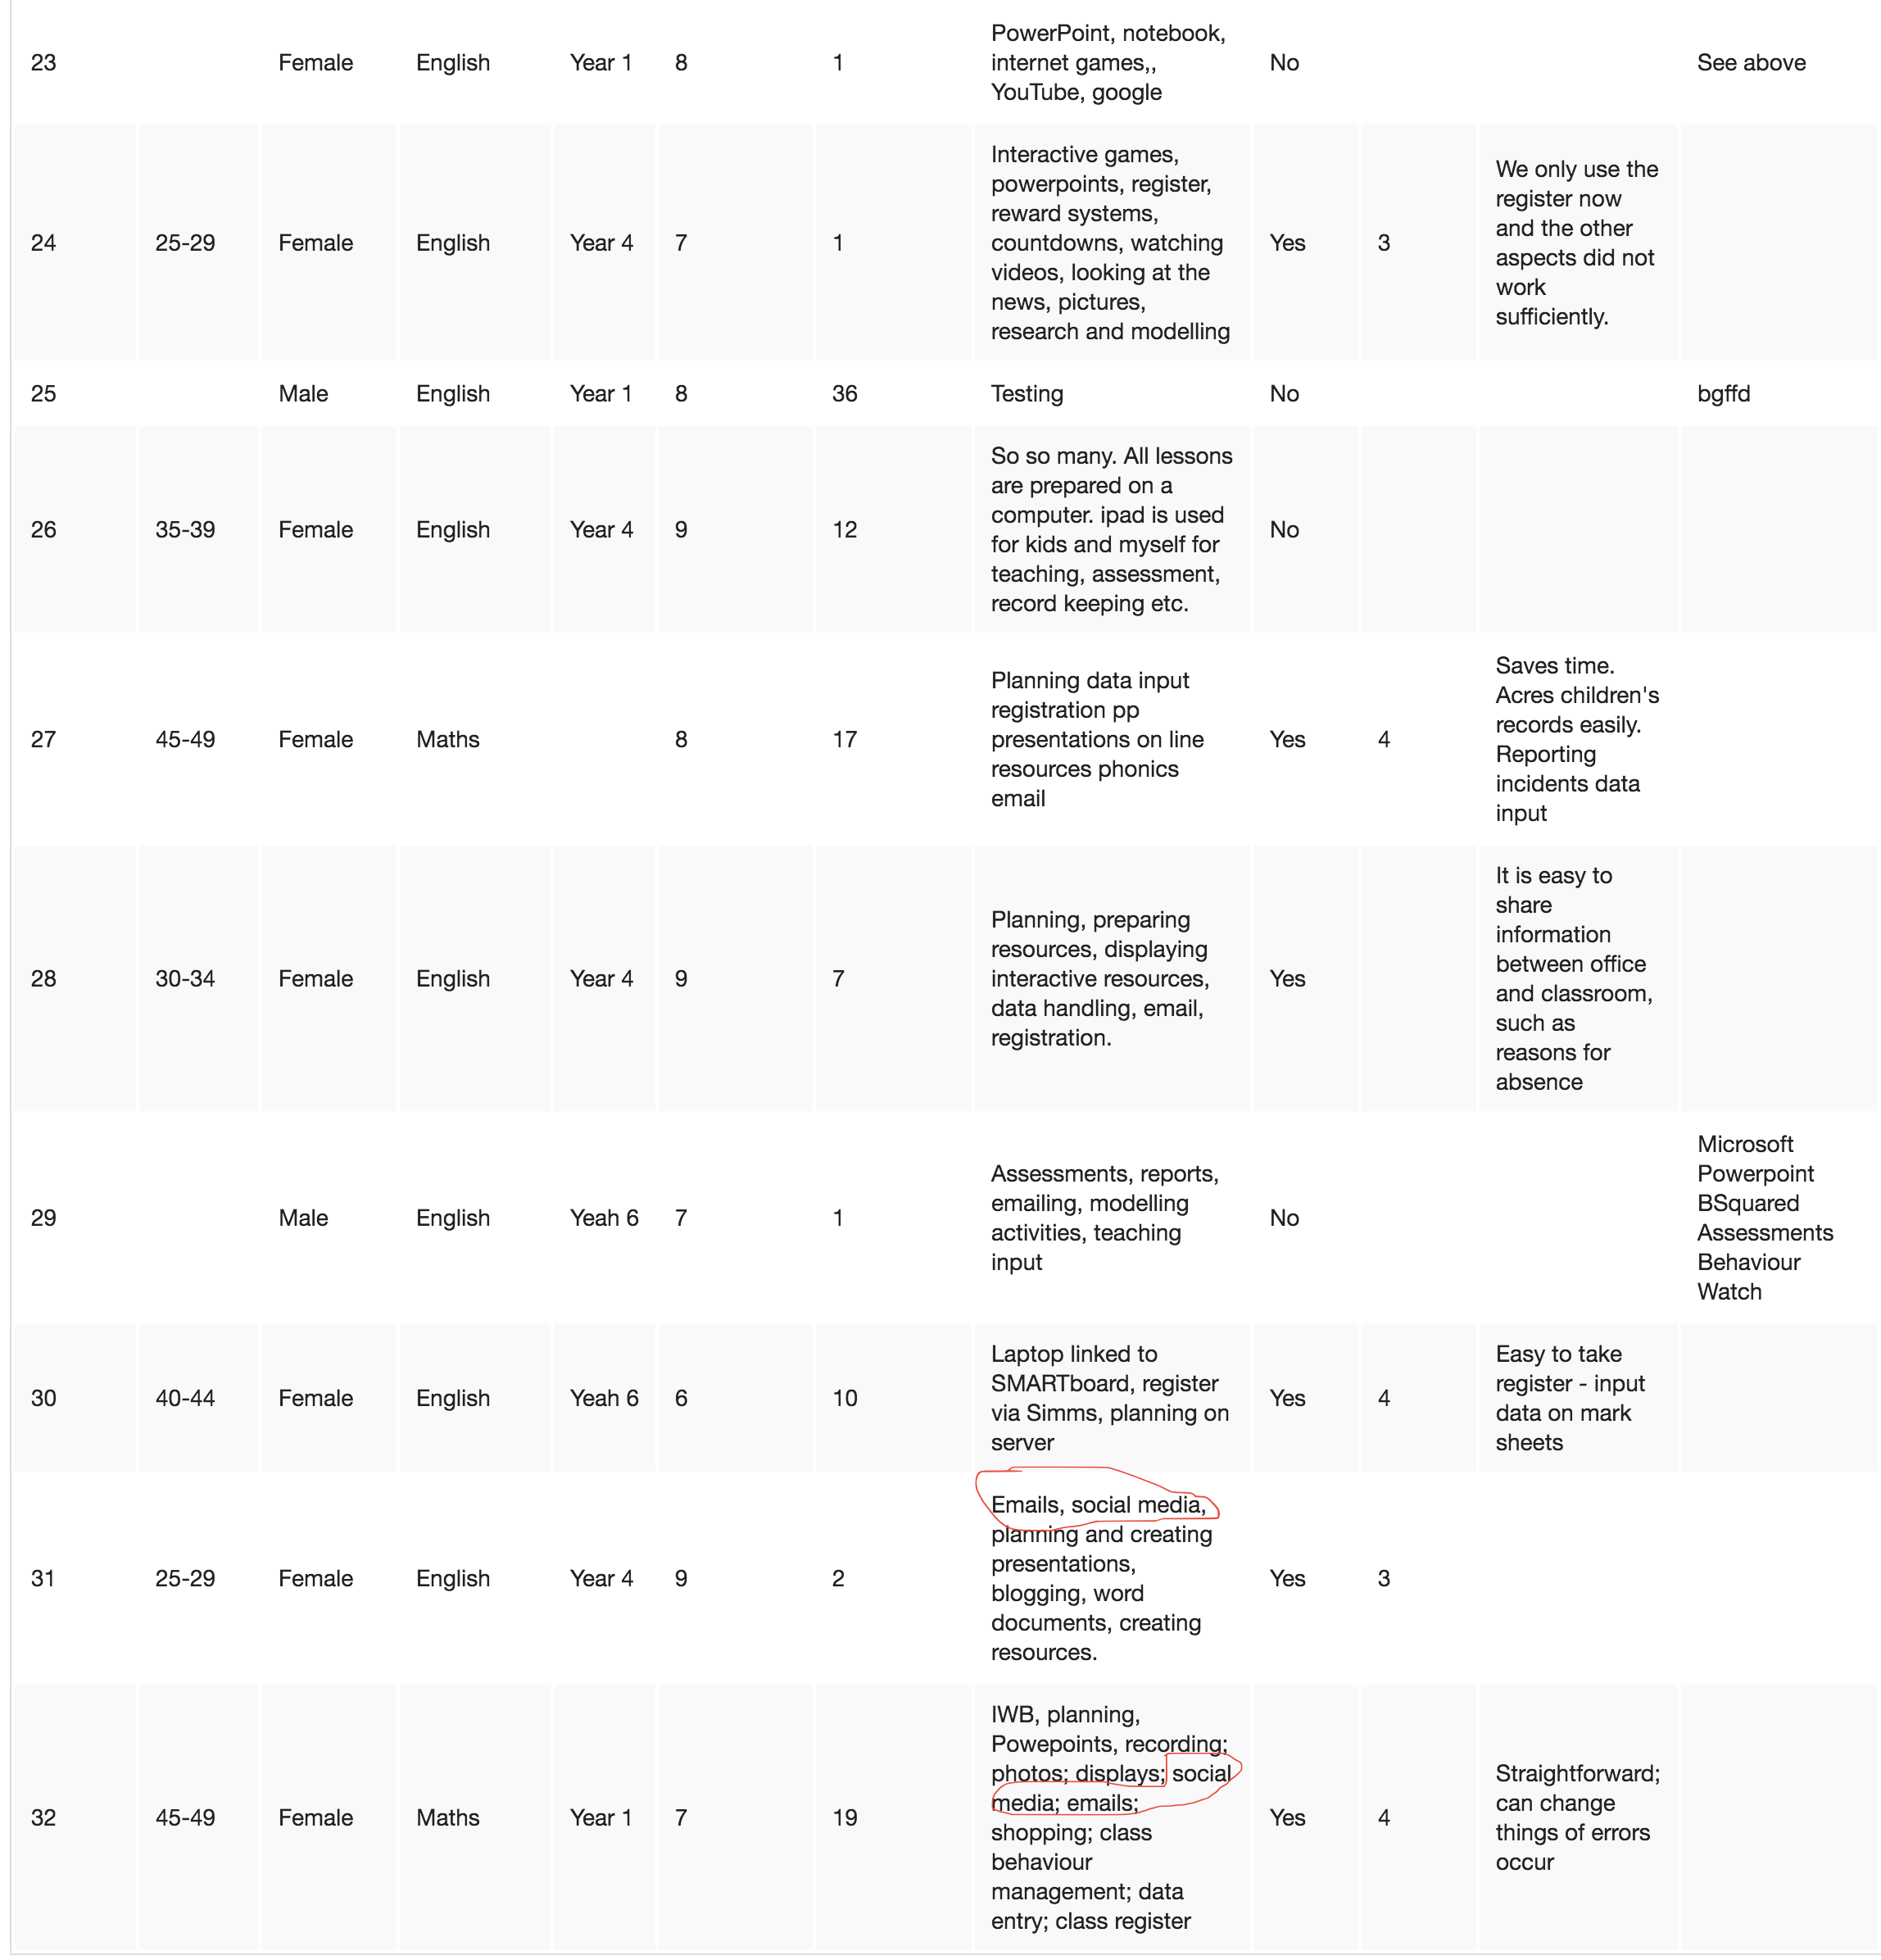
\includegraphics[scale=0.3]{figures/women_stat}
\end{figure}